\documentclass[a4paper,11pt]{article}
\usepackage{url}
\usepackage{hyperref}
\usepackage{listings}
\usepackage{color}
\usepackage{tikz}
\usetikzlibrary{arrows}
\usetikzlibrary{patterns}

\hoffset 0in
\oddsidemargin 0in
\voffset -0.4in
\topmargin 0in
\headheight 12pt
\headsep 0,5in

\marginparwidth 50pt
\marginparsep 5pt
\reversemarginpar


\textwidth 6.5in
\displaywidth 6.5in
\textheight 240mm
\parindent 0mm
\parskip \baselineskip

\newcommand{\code}[1]{\texttt{#1}}

%\newcommand{\heading}[1]{\vspace{2ex}\section*{#1}}
\newcommand{\refsection}[1]{Section \ref{#1}}


\begin{document}

\title{ \bf ENEL464 Embedded Software and Advanced Computing 2021 \\ Group Assignment 2}
\author{}
%\author{Michael Hayes}
\date{}
\maketitle


\section{Introduction}

The purpose of this assignment is to implement a numerical algorithm
on a computer to make the most efficient use of its caches and cores.
You will find that you will get a large variation in program
performance depending on how you implement your code and use compiler
optimisations.  A knowledge of computer architecture should help with
this!

The algorithm is Jacobi relaxation.  This is an iterative algorithm
used to approximate differential equations, for example, Poisson's and
Laplace's equations.  Poisson's equation can be used to find the
electric potential given a specified charge distribution or
temperature given a specified heat source.  There are more efficient
ways to solve this problem using Green's functions and Fourier
transforms but that is not the purpose of this assignment.

\section{Jacobi relaxation}

The discrete form of Poisson's equation is
%
\begin{equation}
  \nabla^2 V_{i,j,k,n} = f_{i,j,k,n},
\end{equation}
%
where $f$ is the source (say, the electric charge) and $V$ is the
potential field to be determined.  Poisson's equation is a partial
differential equation and thus requires boundary conditions.  For the
assignment Neumann boundary conditions are required.  This is
equivalent to enclosing the problem in an insulating box so that no
current flows across the boundary.

Poisson's equation can be solved iteratively, at each time-step $n$,
using Jacobi relaxation, where
%
\begin{equation}
  V_{i,j,k,n+1} = \frac{1}{6} \left(V_{i+1,j,k,n} + V_{i-1,j,k,n} + V_{i,j+1,k,n} + V_{i,j-1,k,n} + V_{i,j,k+1,n} + V_{i,j,k-1,n} - \Delta^2 f_{i,j,k}\right).
\label{eqn:Jacobi}
\end{equation}
%
Here $\Delta = \Delta x = \Delta y = \Delta z$ is the spacing between
voxels in metres, $0 \le i < N$, $0 \le j < N$, and $0 \le k <
N$. Voxels on the boundary ($i = -1$, $i=N$, $j = -1$, $j=N$, $k =
-1$, $k=N$) are defined such that the derivative over that boundary is
zero ($\partial V / \partial n = 0$), see Fig.  \ref{fig:Boundary}.
You might recognise (\ref{eqn:Jacobi}) as a 3-D discrete convolution
at each time-step.

\begin{figure}
  \centering
  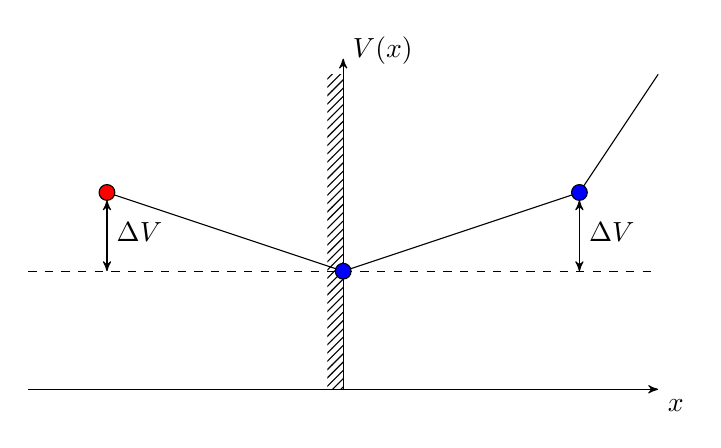
\begin{tikzpicture}
    \tikzset{>=stealth'}

    % Draw some axes
    \draw[->] (-4, 0) -- (4, 0);
    \draw[->] (0, 0) -- (0, 4.2);

    \node[above right] at(0, 4) {$V(x)$};
    \node[below right] at(4, 0) {$x$};

    % Draw the boundary
    \fill[pattern=north east lines]
        (-0.2, 0) -- (-0.2, 4) -- (0, 4) -- (0, 0);

    \draw (-3, 2.5) -- (0, 1.5) -- (3, 2.5) -- (4, 4);

    \draw[dashed] (-4, 1.5) -- (4, 1.5);

    \draw[fill=red] (-3, 2.5) circle (0.1);
    \draw[fill=blue] (0, 1.5) circle (0.1);
    \draw[fill=blue] (3, 2.5) circle (0.1);

    \draw[<->] (-3, 1.5) -- (-3, 2.4);
    \draw[<->] (3, 1.5) -- (3, 2.4);

    \node[right] at (3, 2) {$\Delta V$};
    \node[right] at (-3, 2) {$\Delta V$};
  \end{tikzpicture}
  \caption{Illustration of a Neumann boundary condition where the external
  `ghost' point (red) is defined such that the gradient at the boundary is zero
  with respect to the internal points (blue).}
  \label{fig:Boundary}
\end{figure}


\section{Implementation}

Your program to solve (\ref{eqn:Jacobi}) must either use C or C++.  Your
goal is to find a fast implementation that will run on your (or a CAE
lab) computer, making best use of the caches and multiple cores.

A good starting point is provided with \emph{poisson.c}. You should modify this
to solve the assignment. Instructions on building it are in the source code.
Some suggested reading is located in the \emph{docs/} folder regarding compiler
optimisations, multithreading, and profiling.

% This repository is configured for continuous integration testing on eng-git and
% if you heavily modify the source code, you will need to modify the runner
% instructions to match.


Code templates can be found at
\url{https://eng-git.canterbury.ac.nz/bmi32/464_template_2021}. We recommend
writing your solutions in a Linux-like environment. This means any Linux
distribution, MacOS with Homebrew, or Windows with WSL. Your mileage may vary
with the profiling tools in anything other than Linux.


\section{Testing}

Test your algorithm with a single point charge in the centre of the
volume, i.e.,
%
\begin{equation}
  f_{i,j,k} = \left\{
  \begin{array}{ll}
    1 & i=N/2, j=N/2, k=N/2, \\
    0 & \mbox{otherwise}
  \end{array}\right.,
\end{equation}
%
where the volume is comprised of $N \times N \times N$ voxels.  Note,
you algorithm must work with arbitrary source distributions.

A testing script (\emph{test.sh}) has been provided along with some sample
outputs at several cube sizes. This will automatically compare your output
against a reference implementation.



%% There is a simple explanation of the 2-D algorithm at
%% \url{https://blogs.msdn.microsoft.com/visualizeparallel/2010/03/29/the-jacobi-relaxation-an-instance-of-data-parallelism/}

\section{Support}

Only questions submitted via the ENCE464 assignment forum will be
answered.  Emails will be quietly ignored.


\section{Reports}

The reports are group reports and are to be submitted as PDF documents
through the ENCE464 Learn page.  They will be submitted to TurnItIn
for plagiarism checking.

Guidelines for writing a report are available at\\
\url{https://eng-git.canterbury.ac.nz/mph/report-guidelines/blob/master/report-guidelines.pdf}.

Each report is to use a 12 point font and be no longer than five
pages, including appendices.  Please use margins of at least 2\,cm.

%Ensure in your report that you discuss your implementation in terms of
%cache usage and core usage.  You should present profiling information
%showing which parts of your program takes the most time to execute.

\section{Assessment}

Your report will be marked in terms of:
%
\begin{itemize}
\item Written style.  The writing should be concise technical writing.
\item Presentation.  The key here is consistency and clear diagrams
  and graphs.
\item Architecture overview.  This should describe your computer's
  architecture (such as the cache organisation, memory size, CPU model,
  etc.).
\item Multithreading analysis.  This should discuss how your program
  takes advantage of multiple cores.
\item Cache analysis.  This should discuss how your program takes
  advantage of the cache.
\item Profiling analysis.  This should show which parts of your
  program take the most time.
\item Optimisation analysis.  This should discuss the affects of some
  of the compiler optimisations, such as loop unrolling, on your
  program.
\item Overall excellence.
\end{itemize}
%
Each section is marked out of 5, giving a total of 40 marks.  Five
bonus marks will be awarded to any group who can beat our program when
running on a CAE lab computer and give the correct results.

Your report should present the statistics for the time your program
takes to run for the following problem sizes: $N=101, 201, 301, 401,
501, 601, 701, 801, 901$.  For $N=801$ and $N=901$, do not worry about
performing many trials.  If you have a really old computer, you can
skip $N=901$.

Your analyses should be backed up with experimental evidence, such as
the output from profiling tools.


%% Bonus marks will be awarded for implementations that handle either Neumann or
%% Dirichlet boundary conditions on each boundary. This is equivalent to an
%% insulating layer on the boundary.


\section{Code}

We expect you to use git for version control.  However, you must
submit your code as a \code{.zip} file so it can be checked for
numerical accuracy and plagiarism.  Your fastest implementation must
be able to built by running \code{make}.


\end{document}
